\section{Kiến trúc Module và Luồng Phụ thuộc}
\label{sec:kien-truc-module}

Phần này sẽ phân rã hệ thống thành các khối module logic, trả lời câu hỏi "Dự án gồm những module nào và chúng liên quan đến nhau ra sao?". Việc hiểu rõ cấu trúc module là nền tảng để có thể nắm bắt được cách tổ chức của codebase.

\subsection{Sơ đồ Phụ thuộc Module}
\label{subsec:so-do-phu-thuoc}

Kiến trúc của hệ thống được tổ chức thành các module NestJS riêng biệt, mỗi module chịu trách nhiệm cho một domain nghiệp vụ hoặc một chức năng kỹ thuật cụ thể. Mối quan hệ phụ thuộc (\texttt{imports}) giữa các module này được thể hiện trong Sơ đồ \ref{fig:module-dependencies}.

Sơ đồ này cho thấy \texttt{AppModule} là module gốc, có vai trò lắp ráp tất cả các module khác lại với nhau. Các mũi tên thể hiện một module đang "nhập khẩu" (sử dụng) một module khác. Ví dụ, \texttt{GatewayModule} cần đến \texttt{AuthModule} để xác thực người dùng và cần \texttt{InboxModule} để xử lý các nghiệp vụ liên quan đến tin nhắn.

\begin{figure}[h!]
    \centering
    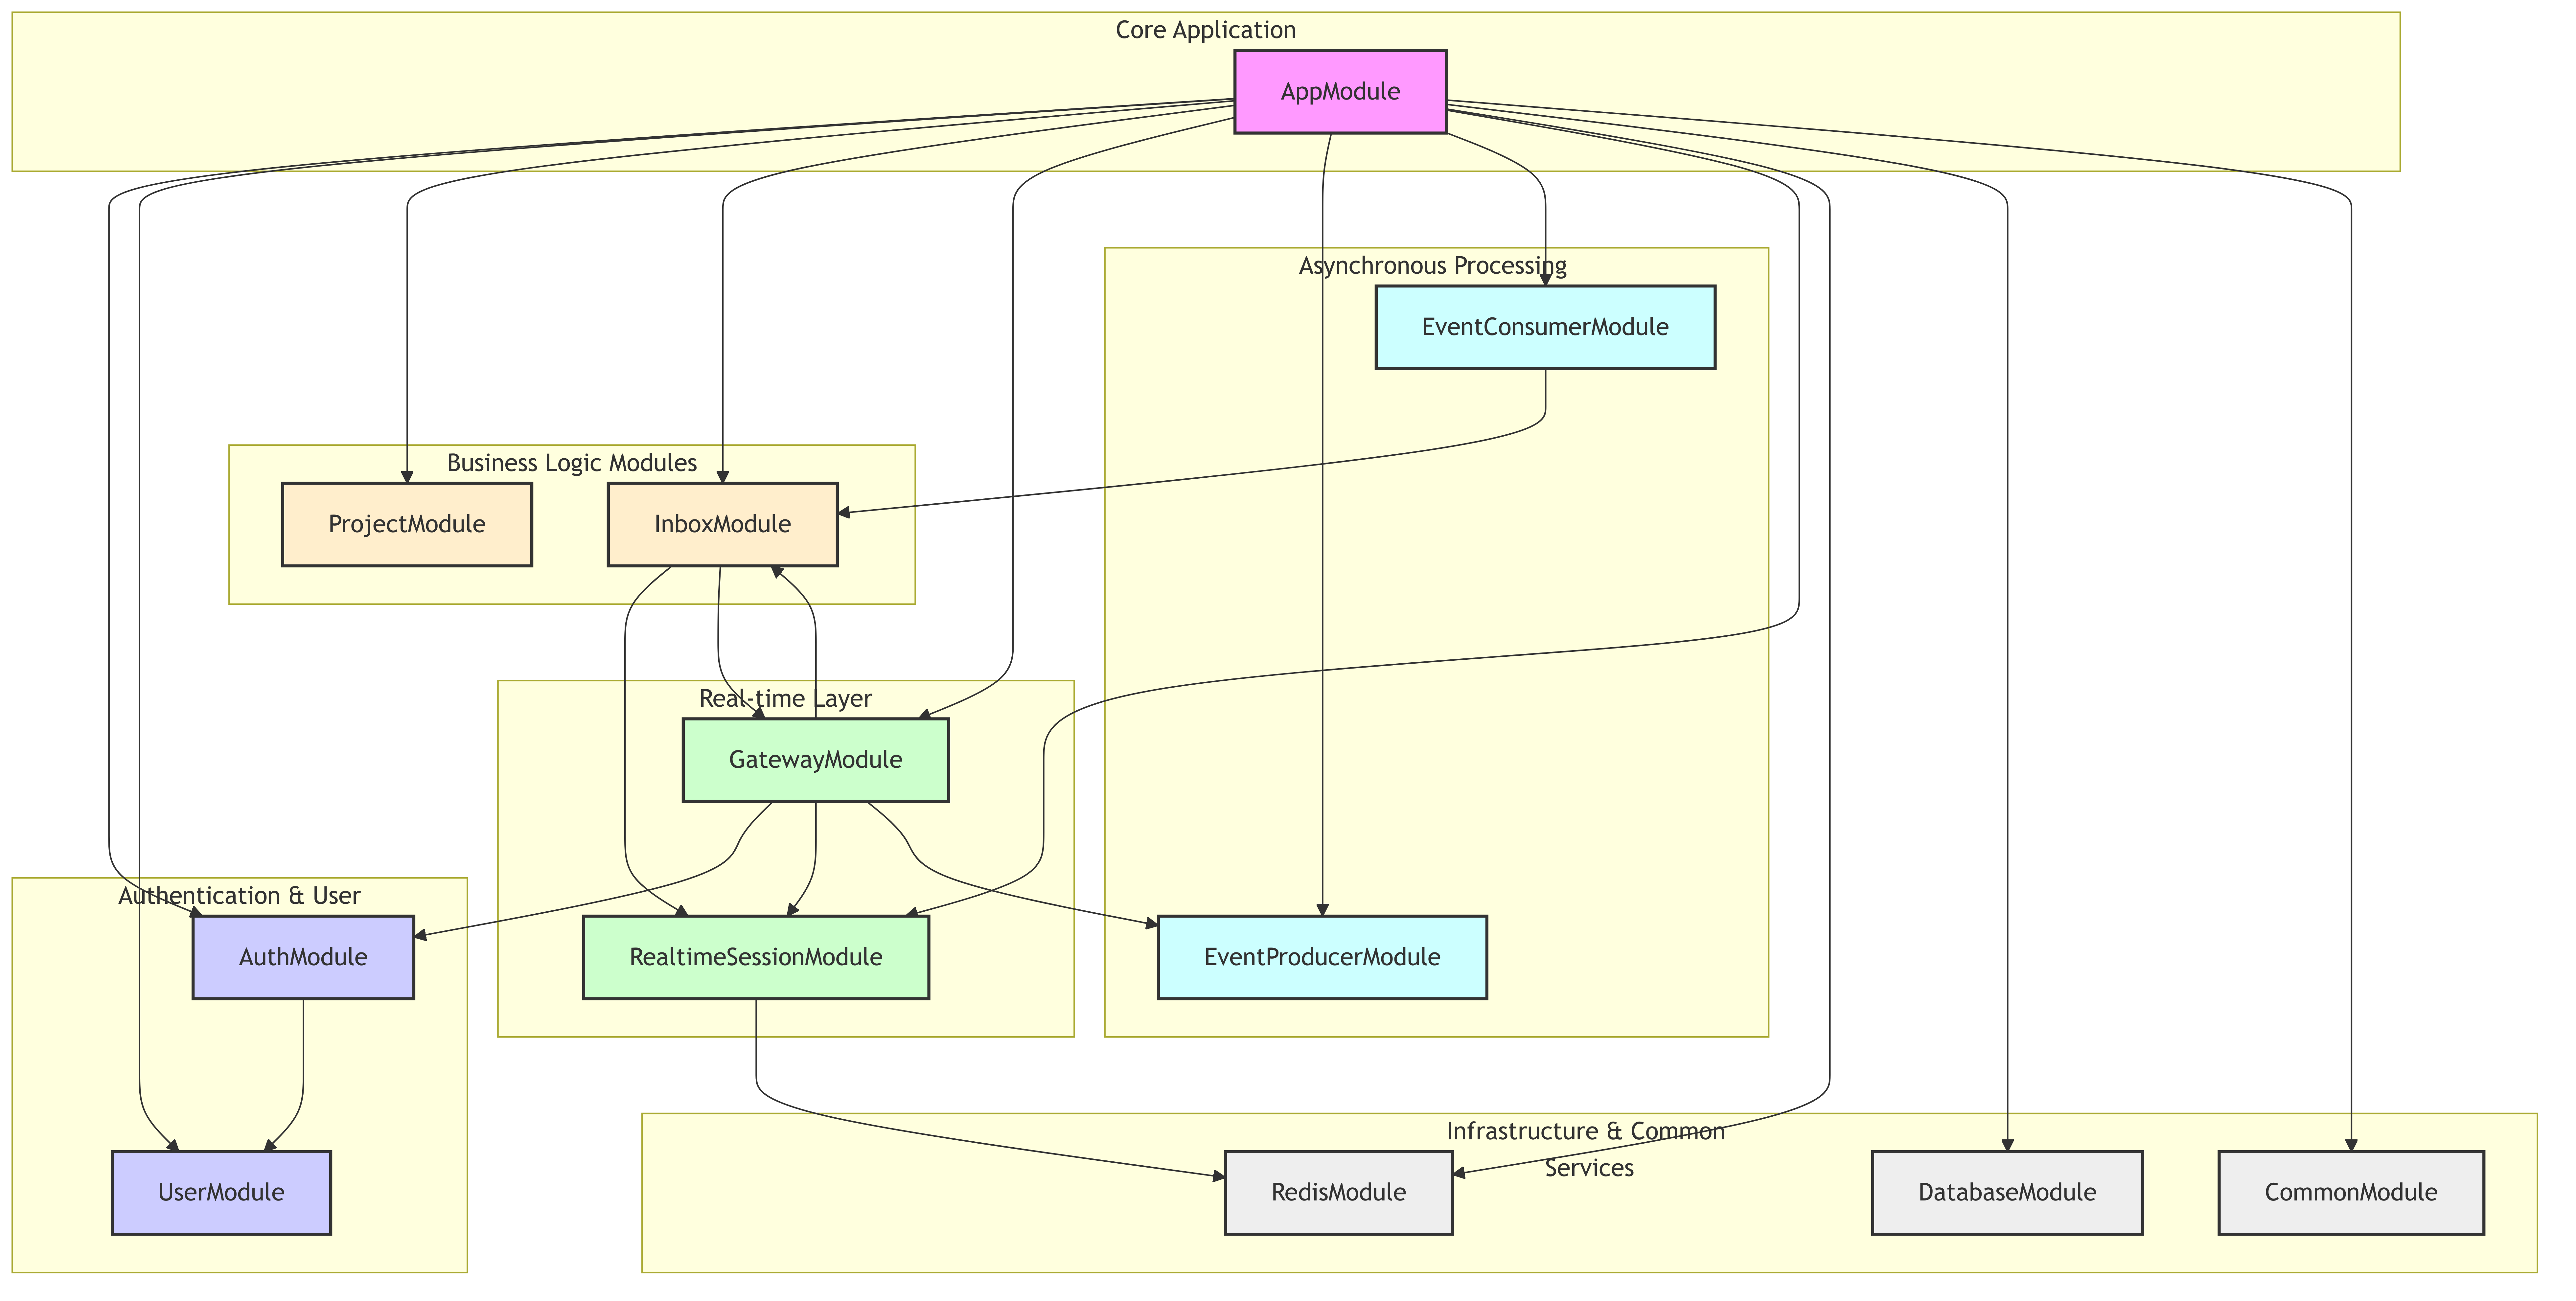
\includegraphics[width=\textwidth]{images/module-relation.png}
    \caption{Sơ đồ Phụ thuộc giữa các Module}
    \label{fig:module-dependencies}
\end{figure}
\subsection{Mô tả các Module Chính}
\label{subsec:mo-ta-module}

Dưới đây là bản tóm tắt về vai trò và trách nhiệm của từng module chính trong hệ thống, giúp làm rõ hơn chức năng của các khối trong Sơ đồ \ref{fig:module-dependencies}.

\begin{itemize}
    \item \textbf{AppModule:} Là module gốc của ứng dụng NestJS. Nó không chứa logic nghiệp vụ mà đóng vai trò là điểm tích hợp, chịu trách nhiệm "lắp ráp" và cấu hình tất cả các module khác để tạo thành một hệ thống hoàn chỉnh.

    \item \textbf{UserModule:} Quản lý tất cả các nghiệp vụ liên quan đến người dùng của hệ thống (ở đây là các nhân viên hỗ trợ - agent). Nó bao gồm các thao tác CRUD (Tạo, Đọc, Cập nhật, Xóa) thông tin người dùng và định nghĩa entity \texttt{User}.
    
    \item \textbf{AuthModule:} Chịu trách nhiệm cho toàn bộ quá trình xác thực và phân quyền. Nó xử lý logic đăng ký, đăng nhập, đổi mật khẩu, đăng nhập qua Google, và quản lý vòng đời của JSON Web Tokens (JWT).

    \item \textbf{ProjectModule:} Quản lý các "Dự án" theo kiến trúc multi-tenant. Module này xử lý các thao tác CRUD cho dự án, quản lý thành viên và vai trò của họ (Manager, Agent), và chứa toàn bộ logic cho hệ thống mời thành viên qua email.
    
    \item \textbf{InboxModule:} Là module nghiệp vụ lớn nhất, chứa toàn bộ logic cốt lõi liên quan đến Hộp thư. Nó quản lý các thực thể và nghiệp vụ của các cuộc hội thoại (\texttt{Conversation}), tin nhắn (\texttt{Message}), và khách truy cập (\texttt{Visitor}).
    
    \item \textbf{GatewayModule:} Là lớp giao tiếp real-time (WebSocket) tinh gọn. Nó không xử lý nghiệp vụ trực tiếp mà sử dụng \texttt{EventEmitter2} để chuyển đổi các sự kiện từ client thành các sự kiện nội bộ, giúp hệ thống luôn phản hồi nhanh và không bị block. Nó cũng lắng nghe Redis Pub/Sub để giao tiếp liên-server.

    \item \textbf{EventProducerModule:} Một module hạ tầng kỹ thuật. Nó cung cấp một service (\texttt{SqsService}) với phương thức \texttt{sendMessage}, cho phép các phần khác của ứng dụng có thể đẩy một tác vụ vào hàng đợi SQS để xử lý bất đồng bộ.
    
    \item \textbf{EventConsumerModule:} Một service chạy nền bên trong ứng dụng chính. Nó không phải là một worker độc lập. Service này khởi động một vòng lặp polling vô hạn để liên tục lấy các tác vụ từ hàng đợi SQS, xử lý chúng (thường là các thao tác ghi CSDL), và sau đó publish kết quả vào một kênh Redis để Gateway có thể nhận và thông báo cho client.

    \item \textbf{RealtimeSessionModule:} Quản lý trạng thái kết nối real-time của các visitor. Nó sử dụng Redis để lưu trữ và tra cứu mối liên kết giữa định danh của visitor (\texttt{visitorUid}) và ID kết nối socket (\texttt{socket.id}) của họ.

    \item \textbf{RedisModule \& DatabaseModule:} Là các module hạ tầng. Chúng cung cấp các kết nối đã được cấu hình sẵn đến Redis và cơ sở dữ liệu PostgreSQL (thông qua TypeORM) cho toàn bộ ứng dụng.
\end{itemize}